% Copyright 2013 Nicolai Hähnle <nhaehnle@gmail.com>
%
% This work is licensed under the Creative Commons Attribution-ShareAlike 3.0
% Unported License, see http://creativecommons.org/licenses/by-sa/3.0/
%
% Among other things, this means that yes, you may take e.g. illustrations from
% the book and use them in your own work. However, (a) you must give proper
% attribution by naming me as its original author and (b) you must make your
% derivative work available under the same or similar license terms.
%
% See the Creative Commons website for the exact licensing terms.

\chapter{The Voronoi Cell of a Lattice and its Applications}

The Voronoi diagram of a point set is defined
to provide the answer to the closest vector problem:
given a point set $P$,
the Voronoi cell of $x \in P$ is the set of points
that are closer to $x$ than to any other point in $P$.

In this chapter, we will see how the Voronoi diagram of a lattice
can be used to solve both the shortest and the closest vector problem
in single exponential time by a deterministic algorithm.
Considering how early Voronoi diagrams were first studied,
and how obvious their usefulness seems in hindsight,
it took a very long to find this algorithm
which is due to Micciancio and Voulgaris~\cite{MR2743283}.


\section{The Voronoi cell of a lattice}

\begin{definition}
  Let $\Lambda \subset \R^d$ be a lattice.
  Let $x \in \Lambda \setminus \{ 0 \}$.
  We define the open half-space
  \[
    H_x := \{ p \in \R^d ~:~ \|p\|_2 < \|x-p\|_2 \}
  \]
  and the (open) \emph{Voronoi cell} of $\Lambda$
  \[
    \cV_\Lambda := \bigcup_{x \in \Lambda\setminus\{0\}} H_x
  \]
\end{definition}

In the following $2$-dimensional example,
the Voronoi cell $\cV_\Lambda$ is shaded.
Its translates $x + \cV_\Lambda$ for $x \in \Lambda$ are shown as well.
\begin{center}
  \begin{tikzpicture}
    \clip (-2.2,-2.3) rectangle (2.2,4.3);

    \fill[black!10]
      (0,1.0625) -- (0.5,0.9375) -- (0.5,-0.9375) -- (0,-1.0625) --
      (-0.5,-0.9375) -- (-0.5,0.9375) --cycle;

    \foreach \y in {-1,0,1,2}
      \foreach \x in {-3,-2,-1,0,1,2}
        \fill ($\x*(1,0) + \y*(0.5,2)$) circle[radius=2pt];

    \draw (0,0) node[below] {$0$};

    \foreach \y in {-1,0,1,2}
      \foreach \x in {-4,-3,-2,-1,0,1,2}
        \draw ($\x*(1,0) + \y*(0.5,2)$) +(0,1.0625) -- +(0.5,0.9375) -- +(0.5,-0.9375) -- +(0,-1.0625);
  \end{tikzpicture}
\end{center}

\begin{lemma}
  If $\Lambda$ is full-dimensional, $\overline{\cV_\Lambda}$ is a polytope.

  For a general lattice $\Lambda$,
  $\overline{\cV_\Lambda} = P + \langle \Lambda \rangle^\bot$
  where $P = \overline{\cV_\Lambda} \cap \langle \Lambda \rangle$ is a polytope.
\end{lemma}
\begin{proof}
  For linearly independent vectors $x_1, \ldots, x_d \in \Lambda$,
  we have
  \[
    \cV_\Lambda \subseteq
      \underbrace{H_{x_1} \cap \dots \cap H_{x_d} \cap H_{-x_1} \cap \dots \cap H_{-x_d}}_{=: Q}.
  \]
  The right hand side $Q$ is an open parallelepiped.
  In particular, it is bounded, so $\cV_\Lambda$ is bounded.

  Let $R > 0$ such that $Q \subseteq B(0,R)$.
  Every facet of $\overline{Q}$ lies on a hyperplane of the form
  \[
    \|p\|_2 = \|x - p\|_2 \iff 2p^Tx = x^Tx
  \]
  for some $x = \pm x_j$.
  Note that $\|p\|_2 \geq \frac{1}{2} \|x\|$ for all points $p$ on the facet.
  On the other hand, $\|p\|_2 \leq R$ by definition of $R$,
  so that we get $\|\pm x_j\|_2 \leq 2R$ for all $j$.

  We claim that
  \[
    \cV_\Lambda = \bigcap_{x \in \Lambda\setminus\{0\} ~:~ \|x\|_2 \leq 2R} H_x
  \]
  follows.
  The inclusion from left to right is clear from the definition.
  For the inclusion from right to left,
  let $p \in H_x$ for all $x \in \Lambda\setminus\{0\}$ with $\|x\|_2 \leq 2R$.
  In particular, this implies $\|x\|_2 \leq R$ by our choice of $R$.
  This in turn implies $x \in H_y$ for all $y$ with $\|y\|_2 > 2R$.
  To summarize,
  \[
     x \in \left( \bigcap_{x \in \Lambda\setminus\{0\} ~:~ \|x\|_2 \leq 2R} H_x \right)
      \cap \left( \bigcap_{y \in \Lambda\setminus\{0\} ~:~ \|y\|_2 > 2R} H_y \right) = \cV_\Lambda
  \]
  which implies the claim.
  That is, $\cV_\Lambda$ is bounded and defined as the intersection of finitely many half-spaces,
  i.e., it is a polytope.

  The statement of the Lemma for general lattices follows
  directly from the observation that $x \in \Lambda$ is a closest lattice vector to $p$
  if and only if it is a closest lattice vector of the orthogonal projection $p'$ of $p$
  onto $\langle \Lambda \rangle$.
\end{proof}

Now that we have established that $\cV_\Lambda$ is a polytope,
a natural algorithmic representation suggests itself:

\begin{definition}
  We say that $x \in \Lambda$ is \emph{Voronoi relevant} if
  \[
    \| p \|_2 \leq \| x - p \|_2 \iff 2p^Tx \leq x^T x
  \]
  is a facet-defining inequality of $\overline{\cV_\Lambda}$.
\end{definition}

Given a representation of $\cV_\Lambda$ in terms of Voronoi relevant vectors,
simple tasks such as testing whether a point is contained in $\cV_\Lambda$
can be solved in time $N \cdot \poly(d, b)$,
where $b$ is the encoding size of the coordinates
and $N$ is the number of Voronoi relevant vectors.
Our first goal in this chapter will be to bound this number $N$.
Before we can do this -- and simultaneously show how those vectors
can be found -- we need some basic tools.

\begin{lemma}
  \label{lemma:voronoi-diagram-symmetry}
  Let $x \in \frac{1}{2} \Lambda$.
  The Voronoi diagram of $\Lambda$ is symmetric with respect to $x$.
\end{lemma}
\begin{proof}
  Since the symmetry $x + u \mapsto x - u$ preserves distances,
  we only need to show that the lattice $\Lambda$ is symmetric with respect to $x$.
  Whenever $x + u \in \Lambda$, we have
  \[
    x - u = (x + u) - 2u,
  \]
  where $u \in \frac{1}{2} \Lambda$.
  That is, $x - u \in \Lambda$ as well, completing the proof.
\end{proof}

\begin{lemma}
  \label{lemma:voronoi-relevant-facet-interior}
  Let $x \in \Lambda$ be a Voronoi relevant vector.
  Then $x/2$ lies in the relative interior of the associated facet of $\cV_\Lambda$.
\end{lemma}
\begin{proof}
  The facet associated to $x$ is
  \[
    F = \cV_\Lambda \cap \{ 2p^x = x^Tx \}
  \]
  The point $x/2$ lies on the hyperplane defining $F$,
  and by Lemma~\ref{lemma:voronoi-diagram-symmetry},
  the entire Voronoi diagram is symmetric with respect to $x/2$.
  In particular, $F$ is symmetric with respect to $x/2$.
  Since $F$ is convex, this implies the claim.
\end{proof}

\begin{lemma}
  \label{lemma:voronoi-relevant-as-closest}
  Let $x \in \Lambda$.
  Then $x$ is Voronoi relevant if and only if
  $0$ and $x$ are the unique closest vectors to $\frac{1}{2} x$.
\end{lemma}
\begin{proof}
  Let $x$ be Voronoi relevant and
  assume that there is a third vector $y \in \Lambda$ that is equally close or closer.
  \begin{center}
    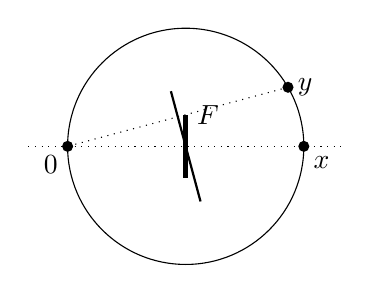
\begin{tikzpicture}
      \fill (0,0) circle[radius=2pt] node[below left] {$0$};
      \fill (3,0) circle[radius=2pt] node[below right] {$x$};
      \draw[dotted] (-0.5,0) -- (3.5,0);
      \draw[ultra thick] (1.5,-0.4) -- (1.5,0.4) node[right] {$F$};
      \draw (1.5,0) circle[radius=1.5cm];

      \fill (1.5,0) +(30:1.5) circle[radius=2pt] node[right] {$y$};
      \draw[thick] (1.5,0) +(0.188,-0.7) -- +(-0.188,0.7);
      \draw[dotted] (2.8,0.75) -- (0,0);
    \end{tikzpicture}
  \end{center}
  In this case, $x/2$ either lies on the hyperplane bounding $H_y$
  or is cut off by that hyperplane entirely.
  In any case, we have a contradiction with Lemma~\ref{lemma:voronoi-relevant-facet-interior}.

  Now suppose $0$ and $x$ are the unique closest vectors to $\frac{1}{2} x$.
  By compactness, there is a neighborhood of $\frac{1}{2} x$
  in the bounding hyperplane $\partial H_x$ that is contained in $\overline{\cV_\Lambda}$.
  This means that there is a facet of $\overline{\cV_\Lambda}$ in $\partial H_x$,
  i.e., $x$ is Voronoi relevant.
\end{proof}



\section{Computing Voronoi relevant vectors}

A different perspective on the statement of Lemma~\ref{lemma:voronoi-relevant-as-closest}
is the following.
The point $x/2$ lies in the refined lattice $\frac{1}{2} \Lambda$,
to which we can associate a natural \emph{parity function},
see Figure~\ref{fig:lattice-refinement-parity} for an illustration:
\begin{align*}
  \sigma : \frac{1}{2} \Lambda &\to G := (\frac{1}{2} \Lambda) / \Lambda \cong (\Z_2)^d \\
                   u &\mapsto u + \Lambda
\end{align*}%
\begin{figure}
  \begin{center}
  \begin{tikzpicture}
    \clip (-1,-1) rectangle (4,3);
    \foreach \p/\color in {{(0,0)}/black,{(0.75,0.15)}/red,{(-0.05,0.85)}/green,{(0.7,1)}/blue}
      \foreach \x in {-1,0,1,2}
        \foreach \y in {-2,-1,0,1,2}
          \path[fill=\color] ($\x*(1.5,0.3) + \y*(-0.1,1.7)$) +\p circle[radius=2pt];
  \end{tikzpicture}
  \end{center}
  \caption{A lattice $\Lambda$ in black and its refinement $\frac{1}{2} \Lambda$
    with parities indicated using different colors.}
  \label{fig:lattice-refinement-parity}
\end{figure}%
The Lemma then says that for every Voronoi relevant vector $x \in \Lambda$,
there is a vector $u \in \frac{1}{2} \Lambda$ of non-zero parity
such that $0$ and $x$ are the unique closest vectors to $u$ in $\Lambda$.
For all vectors $u' \in \frac{1}{2} \Lambda$ with the \emph{same} parity $\sigma(u') = \sigma(u)$,
the relative location of closest vectors in $\Lambda$ is the same.
This suggests the following algorithm for finding Voronoi relevant vectors:
\begin{codebox}
  \Procname{$\proc{VoronoiCell}(\Lambda)$}
  \li $X \gets \emptyset$
  \li \For $U \gets \left((\frac{1}{2} \Lambda) / \Lambda\right) \setminus \{ 0 \}$
  \li \Do $u \gets$ representative of $U$
  \li     $x \gets \proc{CVP}(\Lambda, u)$
  \li     $X \gets X \cup \{ 2(x - u), 2(u - x) \}$
  \li \Return $X$
\end{codebox}
We are purposefully imprecise about how the lattice $\Lambda$ is represented
and how the closest vector problem is to be solved.
For now, the key point is that we can find all Voronoi relevant vectors
by solving $2^d - 1$ closest vector problems:

\begin{lemma}
  \label{lemma:voronoi-cell-computation}
  The set $X$ returned by \proc{VoronoiCell} contains all Voronoi relevant vectors.
\end{lemma}
\begin{proof}
  Let $y \in \Lambda$ be a Voronoi relevant vector.
  By Lemma~\ref{lemma:voronoi-relevant-as-closest},
  the vector $y/2 \in \frac{1}{2}\Lambda \setminus \Lambda$ has exactly two closest vectors,
  $0$ and $y$.

  There is one iteration of $\proc{VoronoiCell}$ in which $\sigma(u) = \sigma(y/2)$
  or, equivalently, $u \equiv y/2 \pmod{\Lambda}$.
  In this iteration, the closest vector subroutine must return
  either $x = u - y/2$ or $x = u + y/2$, see Figure~\ref{fig:voronoi-cell-computation}.
  In both cases, the algorithm adds $y$ and $-y$ to the set $X$.
\end{proof}
\begin{figure}
  \begin{center}
  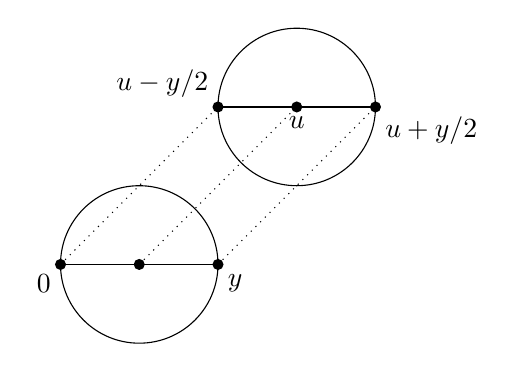
\begin{tikzpicture}
    \fill (0,0) circle[radius=2pt] node[below left] {$0$};
    \fill (2,0) circle[radius=2pt] node[below right] {$y$};
    \fill (1,0) circle[radius=2pt];
    \draw (1,0) circle[radius=1cm];
    \draw (0,0) -- (2,0);

    \fill (3,2) circle[radius=2pt] node[below] {$u$};
    \fill (4,2) circle[radius=2pt] node[below right] {$u + y/2$};
    \fill (2,2) circle[radius=2pt] node[above left] {$u - y/2$};
    \draw (3,2) circle[radius=1cm];
    \draw (2,2) -- (4,2);

    \draw[dotted] (0,0) -- (2,2);
    \draw[dotted] (1,0) -- (3,2);
    \draw[dotted] (2,0) -- (4,2);
  \end{tikzpicture}
  \end{center}
  \caption{Since $u \equiv y/2 \pmod\Lambda$, the set of closest vectors is identical after translation.}
  \label{fig:voronoi-cell-computation}
\end{figure}


\begin{corollary}
  There are at most $2 \cdot (2^d - 1)$ Voronoi relevant vectors.
\end{corollary}



\section{Shortest and closest vectors via the Voronoi cell}

Now that we know how to compute the Voronoi cell,
let us see how it can be used.
First, we see that it contains a list of all shortest vectors of the lattice.

\begin{lemma}
  Let $x \in \Lambda$ be a shortest non-zero vector.
  Then $x$ is Voronoi relevant.
\end{lemma}
\begin{proof}
  Consider the ball of radius $\|x/2\|_2$ around $x/2$:
  \begin{center}
  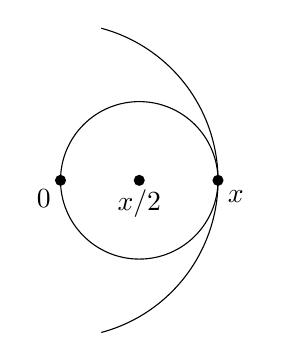
\begin{tikzpicture}
    \fill (0,0) circle[radius=2pt] node[below left]{$0$};
    \fill (2,0) circle[radius=2pt] node[below right]{$x$};
    \fill (1,0) circle[radius=2pt] node[below]{$x/2$};

    \draw (1,0) circle[radius=1cm];
    \draw (0,0) +(-75:2cm) arc[start angle=-75,end angle=75,radius=2cm];
  \end{tikzpicture}
  \end{center}
  Clearly, $0$ and $x$ are the unique closest vectors to $x/2$.
  By Lemma~\ref{lemma:voronoi-relevant-as-closest}, $x$ is Voronoi relevant.
\end{proof}

\begin{corollary}
  Every lattice has at most $2 \cdot (2^d - 1)$ Voronoi relevant vectors.
\end{corollary}
%TODO: kissing number, etc.

We can also use the Voronoi cell to compute closest vectors.
This may seem absurd at first,
because we needed to compute closest vectors in the first place to be able to
find the Voronoi relevant vectors.
However, if we need to solve \emph{many} closest vector problems,
then it turns out to be useful to compute the Voronoi cell first.
We will apply this idea in the Section~\ref{sec:voronoi-full-algorithm}.

For now, suppose we know the Voronoi cell $\cV$ of a lattice $\Lambda$
and are given a target vector $t \in \R^d$.
\begin{center}
  \begin{tikzpicture}
    \clip (-2.2,-2.3) rectangle (2.2,4.3);

    \foreach \y in {-1,0,1,2}
      \foreach \x in {-3,-2,-1,0,1,2}
        \fill ($\x*(1,0) + \y*(0.5,2)$) circle[radius=2pt];

    \draw (0,0) node[below] {$0$};

    \foreach \y in {-1,0,1,2}
      \foreach \x in {-4,-3,-2,-1,0,1,2}
        \draw ($\x*(1,0) + \y*(0.5,2)$) +(0,1.0625) -- +(0.5,0.9375) -- +(0.5,-0.9375) -- +(0,-1.0625);

    \coordinate (t) at (-1.1,3.7);
    \fill (t) circle[radius=2pt] node[left] {$t$};
    \draw (0,0) -- (t);
  \end{tikzpicture}
\end{center}
The problem of finding a closest lattice vector to $t$
is essentially the problem of finding the Voronoi cell translate that contains $t$.
We will solve that problem by following the line segment $[0,t]$.
\begin{codebox}
  \Procname{$\proc{CVP-via-Voronoi-Simple}(\Lambda, \cV_\Lambda, t)$}
  \zi $\cV_\Lambda$ is given by a list that contains all Voronoi relevant vectors
  \li $x \gets 0$
  \li \While $t \not\in x + \overline{\cV_\Lambda}$
  \li \Do Find the point $p$ where $[0,t]$ leaves $x + \cV_\Lambda$
  \li     Let $x' + \cV_\Lambda$, $x' \in \Lambda$, be the Voronoi cell entered at $p$
  \li     $x \gets x'$
      \End
  \li \Return $x$
\end{codebox}
Clearly, the algorithm terminates and returns a correct result.
Each of the individual steps in this algorithm can be implemented in time $O(N \cdot \poly(d,b))$,
where $N$ is the size of the given list containing the Voronoi relevant vectors.
The test whether $t \in x + \overline{\cV_\Lambda}$ can be done by evaluating the $N$ linear functions
associated with the facets of $\overline{\cV_\Lambda}$.
Similarly, the point $p$ and the facet it lies on can be found by intersecting the line through $0$ and $t$
with each of the hyperplanes defining the facets of $x + \overline{\cV_\Lambda}$.

There is a subtle degenerate situation when the segment $[0,t]$ intersects a lower-dimensional
face of a cell $x + \overline{\cV_\Lambda}$.
This degeneracy can be avoided by an appropriate perturbation of the target vector $t$.

For now, let us simply assume that this degenerate situation does not happen
and continue bounding the running time of the algorithm.
Since the Voronoi cells are convex, every cell is entered at most once.
Since we only enter cells that intersect the segment $[0,t]$,
it suffices to bound the number of such cells.

For every $x + \cV_\Lambda$ encountered in the algorithm,
we have $x \in [0,t] + \cV_\Lambda$
and therefore
\[
  x + \cV_\Lambda \subseteq [0,t] + 2 \cV_\Lambda
\]
Since the open cells are disjoint,
it suffices to bound the volume of $[0,t] + 2 \cV_\Lambda$.
\begin{lemma}
  Let $\lambda \in \R$ such that $t \in \lambda \cV_\Lambda$.
  Then \proc{CVP-via-Voronoi-Simple} visits at most $(\lambda+2)^d$ Voronoi cells of the lattice.
\end{lemma}
\begin{proof}
  By convexity, we have $[0,t] \subseteq \lambda \cV_\Lambda$,
  so that
  \[
    x + \cV_\Lambda \subseteq (\lambda + 2) \cV_\Lambda
  \]
  for every Voronoi cell visited by the algorithm.
  Hence, the number of such cells is bounded by
  \[
    \frac{\vol((\lambda + 2) \cV_\Lambda)}{\vol(x + \cV_\Lambda)}
      = \frac{(\lambda + 2)^d \vol \cV_\Lambda }{\vol \cV_\Lambda}
      = (\lambda + 2)^d \qedhere
  \]
\end{proof}
This seems to be a rather crude bound.
Intuitively, we expect a bound that is linear in the norm of $t$ for very large $t$.
But note that even such a bound -- and it is clear that we cannot possibly do better --
is exponential in the encoding size of $t$, which leads to an unacceptable running time.
The solution lies in geometric scaling, using two simple observations.
\begin{corollary}
  If $t \in 2\cV_\Lambda$,
  \proc{CVP-via-Voronoi-Simple} can be used to solve CVP in time $2^{O(d)} \poly(b)$.
\end{corollary}
The second observation is that the Voronoi cell of $k \Lambda$ is simply $k \cV_\Lambda$.

\begin{codebox}
  \Procname{$\proc(CVP-via-Voronoi-Scaling)(\Lambda, \cV_\Lambda, t)$}
\end{codebox}





\section{A single exponential time algorithm for computing the Voronoi cell}
\label{sec:voronoi-full-algorithm}


\section*{Exercises}

\begin{enumerate}
  \item
    \begin{enumerate}[(a)]
    \item Show that $(\frac{1}{2} \Lambda) / \Lambda \cong (\Z_2)^d$.

    \item Show that $|(\Z_2)^d| = 2^d = \frac{\det\Lambda}{\det \frac{1}{2} \Lambda}$.
    \end{enumerate}
\end{enumerate}
